%%%%%%%%%%%%%
% 
% Alexander Powell
% Finite Automata
% Homework Assignment #11
% 12.01.2015
% 
%%%%%%%%%%%%%

\documentclass[11pt]{article}

\usepackage{times,mathptm}
\usepackage{pifont}
\usepackage{exscale}
\usepackage{latexsym}
\usepackage{amsmath}
\usepackage{amssymb}
\usepackage{amsthm}
\usepackage{epsfig}
\usepackage{tikz}
\usepackage{enumerate}
\usepackage{array}
\usepackage{lipsum}
\usepackage{graphicx}
\usepackage{hyperref}


\textwidth 6.5in
\textheight 9in
\oddsidemargin -0.0in
\topmargin -0.0in

\parindent 0pt     % How much the first word of a paragraph is indented. 
\parskip 0pt	   % How much extra space to leave between paragraphs.

\begin{document}

\begin{center}             % If you're only centering 1 line use \centerline{}
\begin{LARGE}
{\bf Finite Automata Homework 11}
\end{LARGE}
\vskip 0.25cm      % vertical skip (0.25 cm)

Due: Tuesday, Dec 1 \\  % force new line
Alexander Powell
\end{center}

\begin{enumerate}[1]

\item Show that the Post Correspondence Problem is decidable over the unary alphabet $\Sigma = \{ 1 \}$.  

\textbf{Solution: }
\begin{proof}

In the Post Correspondence Problem using a unary alphabet, we deal with tiles of the form  $\Bigg[ \dfrac{1^i}{1^j} \Bigg]$.  Now, the tiles can take one of three forms: $\Bigg[ \dfrac{1^i}{1^i} \Bigg]$, $\Bigg[ \dfrac{1^i}{1^j} \Bigg]$ where $i>j$, or $\Bigg[ \dfrac{1^i}{1^j} \Bigg]$ where $i<j$.  

\begin{enumerate}
\item In the case where the tiles are of the form $\Bigg[ \dfrac{1^i}{1^i} \Bigg]$, it's simple to find a match so we can accept.  

\item In the case where tiles are of the form $\Bigg[ \dfrac{1^i}{1^j} \Bigg]$ where $i>j$, meaning the number of 1s on the top is greater than the number of 1s on the bottom, then we can't find a match so we reject.  

\item Similarly, if the tiles are of the form $\Bigg[ \dfrac{1^i}{1^j} \Bigg]$ where $i<j$ we reject as well because we can't find a match when there are more 1s on the botton than on the top.  
\end{enumerate}

Therefore, we have shown that the PCP problem is decidable over the unary alphabet $\Sigma = \{ 1 \}$.  

\end{proof}

\newpage

\item This problem considers an attempt at a polynomial reduction from one problem to another that does not work. Your task is to find the flaw. A bipartite graph is an undirected graph in which every cycle has even length. We attempt to show that the Hamiltonian cycle (a cycle that passes through each node exactly once) problempolynomially reduces to the Hamiltonian cycle problem in bipartite graphs. We need a function $T$: \{graphs\}$\rightarrow$\{bipartite graphs\}such that T can be computed in polynomial time and for any graph $G$,$G$ has Hamiltonian cycle iff $T(G)$ has a Hamiltonian cycle. Let $T(G)$ be the bipartite graph obtained by inserting a new vertex on every edge. What is wrong with this transformation?

\textbf{Solution: }
\begin{proof}

To see more clearly what's going wrong with the transformation, we look at a counterexample.  Let's evaluate some graph $G$ that can be shown to have a Hamiltonian cycle.  The graph $G$ is shown below:
\begin{center}
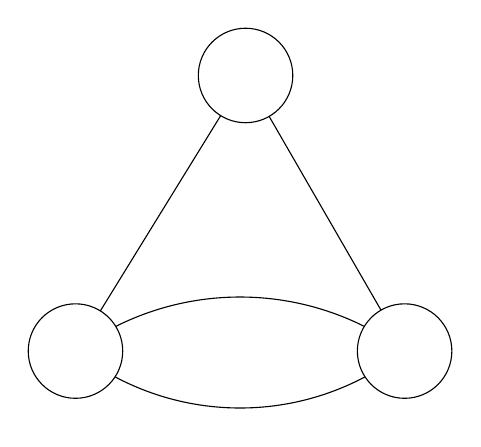
\begin{tikzpicture}[scale=0.2]
\tikzstyle{every node}+=[inner sep=0pt]
\draw [black] (37.1,-12.9) circle (3);
\draw [black] (26.3,-30.4) circle (3);
\draw [black] (47.2,-30.4) circle (3);
\draw [black] (27.88,-27.85) -- (35.52,-15.45);
\draw [black] (45.7,-27.8) -- (38.6,-15.5);
\draw [black] (28.855,-28.835) arc (116.60988:63.39012:17.626);
\draw [black] (44.69,-32.036) arc (-61.98703:-118.01297:16.906);
\end{tikzpicture}
\end{center}

However, we can construct a graph $T(G)$, which is displayed below: \\
\begin{center}
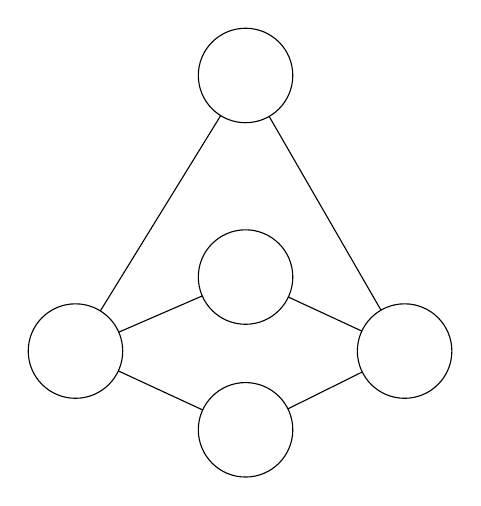
\begin{tikzpicture}[scale=0.2]
\tikzstyle{every node}+=[inner sep=0pt]
\draw [black] (37.1,-12.9) circle (3);
\draw [black] (26.3,-30.4) circle (3);
\draw [black] (47.2,-30.4) circle (3);
\draw [black] (37.1,-25.7) circle (3);
\draw [black] (37.1,-35.4) circle (3);
\draw [black] (27.88,-27.85) -- (35.52,-15.45);
\draw [black] (45.7,-27.8) -- (38.6,-15.5);
\draw [black] (29.05,-29.2) -- (34.35,-26.9);
\draw [black] (39.82,-26.97) -- (44.48,-29.13);
\draw [black] (29.02,-31.66) -- (34.38,-34.14);
\draw [black] (39.79,-34.07) -- (44.51,-31.73);
\end{tikzpicture}
\end{center}

Here, we can clearly see that $T(G)$ does not have a hamiltonian path because there exists no cycle (meaning starting and stopping at the same node) that crosses each node only once.  

Therefore, we can see what is wrong with the transformation and see that it is flawed.  
\end{proof}

\newpage

\item The problem X is defined as follows: \\ INSTANCE: Finite sets $A_1,\ldots,A_m$ and $B_1,\ldots,B_n$. \\ QUESTION: Is there a set $T$ such that $|T\cap A_i|\ge 1$for $i=1,\ldots,m$ and $|T\cap B_j|\le 1$ for $j=1,\ldots,n$? \\ Show that SAT polynomially reduces to X.

\textit{Note: I references the following page to complete this problem:}

\url{http://research.cs.queensu.ca/~cisc365/2010F/365%20SetIntersectionNPC.pdf}

\textbf{Solution: }
\begin{proof}

We say the input to SAT consists of $U$ literals which themselves are distributed among $V$ clauses.  Also, the number of boolean variables in $W$.  Using these variables, we can define a transformation $T$ such that:

\begin{enumerate}
\item For each clause $i$ in $A_i$, we discard logical operators.  We then turn each unnegated literal $x_i$ into a set element $T_i$ and we turn each negated literal $\overline{x_i}$ into a new set element $F_i$.  This is done for all clauses $1 \leq i \leq V$.  It should be noted that $m=V$ in the SAT problem.  

\item We define new elements $B_j = \{ T_j, \text{ } F_j \}$ where $1 \leq j \leq W$.  Here $n=W$, or the number of boolean variables in the SAT problem.  

\end{enumerate}

\end{proof}

\end{enumerate}

\end{document}




































